\documentclass{hnureport}
\usepackage{xeCJK} %调用 xeCJK 宏包
\setCJKmainfont{SimSun} %设置 CJK 主字体为 SimSun (宋体

\renewcommand{\abstractname}{\large Abstract\\}%重定义摘要二字的大小
\begin{document}
\begin{titlepage}
    \clearpage\thispagestyle{empty}
    \centering
    \vspace{1cm}
    % Titles
    {\
        \textsc{Introduction To The Theory Of Computation Michael Sipser}
    }
    \vspace{2.5cm}
    
    \rule{\linewidth}{2mm} \\[0.5cm]
    { \Huge \bfseries Introduction To The Theory Of Computation Michael Sipser\\[0.2em]
        计算理论导论}\\[0.5cm]
    \rule{\linewidth}{0.6mm} \\[1.5cm]
    
    \hspace{2cm}
    \begin{tabular}{l p{5cm}}
        \textbf{Name} & 屈 德 林 \\[10pt]
        \textbf{Student No.} & 201808010522 \\[10pt]
        \textbf{Class} & 计算机科学与技术 1805 \\[10pt]
        \textbf{Department} & CSEE \\[10pt]
        \textbf{Email} & \texttt{qdl.cs@qq.com} \\[10pt]
        \textbf{Date} & \today \\            
    \end{tabular}
    
    % logo
    \vfill
    \centering 
\includegraphics[height=3.5cm]{Figure/bit_logo.png}\\ % light logo
    \centering 
\includegraphics[scale=0.3]{Figure/logo_slogan.png}
    \vspace{0.5cm}

    \pagebreak
\end{titlepage}
    
% \begin{abstract}




\end{abstract}

\noindent\textbf{关键词:} 中美贸易摩擦 \quad  中美关系 \quad 湖南大学 \LaTeX
\newpage    %摘要
\thispagestyle{empty}
\tableofcontents
\newpage 
\setcounter{page}{1}
% 实验目的:Target
\section{Lab Target 目标}
\subsection{数据库定义}
理解和掌握数据库DDL语言,能够熟练地使用SQL DDL语句创建、修改和删除数据库、模式和基本表。
\subsection{数据基本查询}
掌握SQL程序设计基本规范,熟练运用SQL语言实现数据基本查询,包括单表查询、分组统计查询和连接查询。
\subsection{数据高级查询}
掌握SQL程序设计基本规范,熟练运用SQL语言实现数据基本查询,包括单表查询、分组统计查询和连接查询。
\subsection{数据更新}
熟悉数据库的数据更新操作,能够使用SQL语句对数据库进行数据的插入、修改、删除操作。
\subsection{视图}
熟悉SQL语言有关视图的操作,能够熟练使用SQL语句来创建需要的视图,定义数据库外模式,并能使用所创建的视图实现数据管理。 
\subsection{索引}
掌握索引设计原则和技巧,能够创建合适的索引以提高数据库查询、统计分析效率。 
% 实验环境:Environment
\section{Lab Environment 环境}
\begin{itemize}
    \item 操作系统:Arch Linux
    \item 程序运行环境:Python3.7
    \item Python库(标准库未列出):numpy, pandas, matplotlib, sklearn
    \item 报告编写环境:TeX Live 2020
    \item 开发工具: VSCode
\end{itemize}
% 实验内容:Contents
\section{Lab Contents 内容}
\subsection{内容和要求}
理解和掌握SQL DDL语句的语法,特别是各种参数的具体含义和使用方法;使用SQL语句创建、修改和删除数据库、模式和基本表。掌握SQL语句常见语法错误的调试方法。
\subsection{实验重点和难点}
\subsubsection{实验重点}
创建数据库、基本表。
\subsubsection{实验难点}
创建基本表时,为不同的列选择合适的数据类型,正确创建表级和列级完整性约束,如列值是否允许为空、主码和外码等。注意:数据完整性约束,可以在创建基本表时定义,也可以先创建表然后定义完整性约束;由于完整性约束的限制,被引用的表要先创建。
% 实验步骤:Steps
\section{Lab Steps 步骤}
\subsection{实验要求}
理解和掌握SQL DDL语句的语法,特别是各种参数的具体含义和使用方法;使用SQL语句创建、修改和删除数据库、模式和基本表。掌握SQL语句常见语法错误的调试方法。
\subsection{Step1}
创建数据库
CRAETE DATABASE test;
\subsection{Step2}
删除数据库
DROP DATABASE test;
\subsection{Step3}
SQL中创建模式的语句:CRAETE SCHEMA <模式名> AUTHORIZATION <用户名>;
SQL中删除模式的语句:DROP SCHEMA <模式名><CASCADE|RESTRICT>
但是MySQL中没有模式,因此无法创建。
\subsection{Step4}
创建表
CREATE TABLE Student(Sno CHAR(9) PRIMARY KEY,Sname CHAR(20) UNIQUE,Ssex CHAR(2),Sage SMALLINT, Sdept CHAR(20));
Create Table Course(Cno char(4) primary key,Cname Char(40) not null,Cpno char(4),Ccredit smallint,foreign key(Cpno) references Course(Cno));
Create table SC(Sno char(9),Cno char(4),Grade Smallint,primary key(Sno,Cno),foreign key(Sno) references Student(Sno),foreign key (Cno) references Course(Cno));
\subsection{Step5}
删除表
DROP table Student;


% 实验结果:Results
\section{Lab Results 结果}
\subsection{实验结果}
\begin{figure}[htbp]
	\centering
    \subfigure[子图\#1]{
        \label{fig:sub1}		
		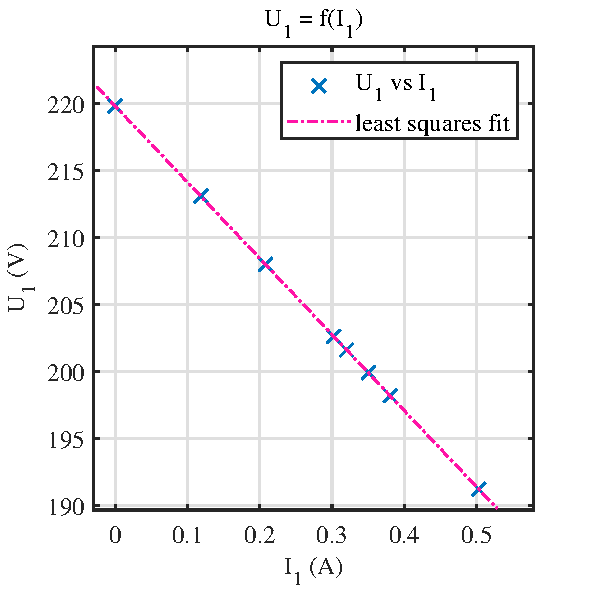
\includegraphics[width=0.45\textwidth]{Figure/fig1.pdf}
    }
    \subfigure[子图\#2]
	{
		\label{fig:sub2}		
		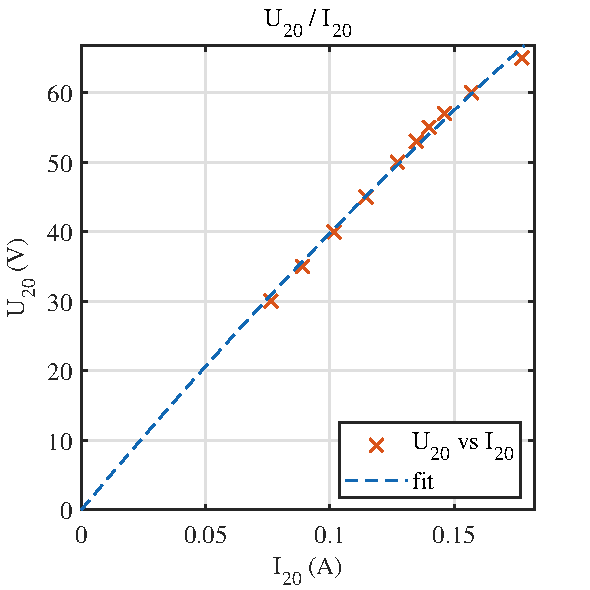
\includegraphics[width=0.45\textwidth]{Figure/fig2.pdf}
	}
	\caption{这里是子图(subfigure)的示例。}
	\label{fig:subfigure}
\end{figure}
通过图像我们发现......,因此我们可以认为....
% 实验心得:Experience
\section{Lab Experience 心得}
\subsection{实验心得a}
理解和掌握SQL DDL语句的语法,特别是各种参数的具体含义和使用方法;使用SQL语句创建、修改和删除数据库、模式和基本表。掌握SQL语句常见语法错误的调试方法。
\subsection{实验心得2}
通过此次试验我熟悉了很多数据库的基本操作,令我收获颇丰


% 引用
\newpage
\begin{thebibliography}{99}
	\bibitem{1}\url{https://www.google.com/}
\end{thebibliography}

\appendix

% 附录
\newpage
\section{附录1:matlab Code}
\begin{lstlisting}[language=matlab]
[X, Y] = meshgrid(0.01:0.01:1, 0.01:0.01:1); 
Zfun =@(x,y)12.5*x.*log10(x).*y.*(y-1)+exp(-((25 ... 
*x - 25/exp(1)).^2+(25*y-25/2).^2).^3)./25; 
Z = Zfun(X,Y); 
figure; 
surf(Y,Z,X,'FaceColor',[1 0.75 0.65],'linestyle','none'); 
hold on 
surf(Y+0.98,Z,X,'FaceColor',[1 0.75 0.65],'linestyle','none'); 
axis equal; 
view([116 30]); 
camlight; 
lighting phong; % 设置光照和光照模式
\end{lstlisting}

\section{附录2:python Code}
\begin{lstlisting}[language=python]
def run():
from sko.GA import GA_TSP
import numpy as np
from scipy import spatial
from numpy.linalg import norm
import cvxpy as cp
import pandas as pd 
#python原始代码
data=pd.read_excel("3.xlsx")
\end{lstlisting}


\end{document}
